
\section{Project Timeline and Gantt Chart}

\begin{figure}[h!]
    \centering
    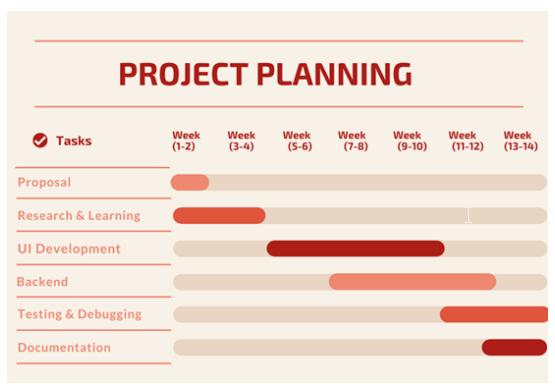
\includegraphics[width=\textwidth]{figures/gantt.png}
    \caption{Gantt Chart}
    \label{fig:gantt_chart}
\end{figure}

\section{Additional Figures and Screenshots}

\begin{figure}
    \centering
    
\includegraphics[width=0.5\linewidth]{selection.png}
    \caption{Model Selection}
    \label{fig:placeholder}
\end{figure}

\begin{figure}[h!]
    \centering
    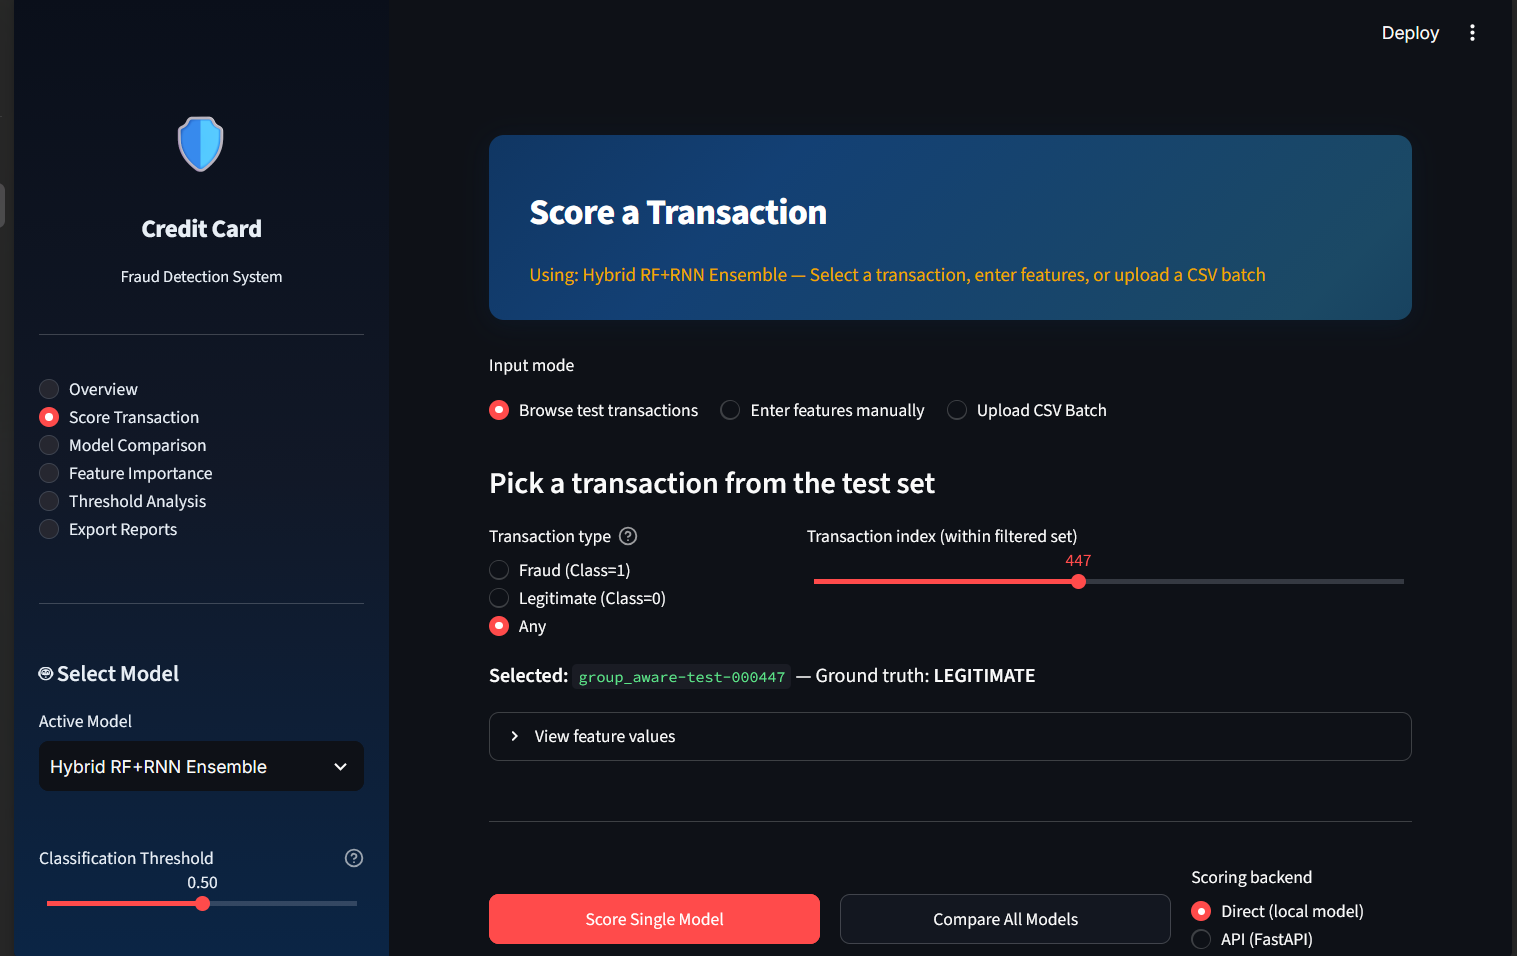
\includegraphics[width=\textwidth]{figures/fraudtransactionscore.png}
    \caption{Fraud Transaction Score}
    \label{fig:homepage}
\end{figure}



\chapter*{Appendix}


\section{User Manual and Installation Guide}

This section describes how to install dependencies, run the training pipeline, and launch the web dashboard and REST API.

\subsection{Prerequisites}
Ensure Python 3.10+ is installed. In a terminal, verify:
\begin{verbatim}
python --version
\end{verbatim}

\subsection{Setup and Installation}
Run the following commands in the project root folder:
\begin{enumerate}
    \item Create a virtual environment:
    \begin{verbatim}
    py -m venv .venv --clear
    \end{verbatim}
    \item Install all required dependencies:
    \begin{verbatim}
    .\.venv\Scripts\python.exe -m pip install pandas numpy pyarrow 
    scikit-learn joblib xgboost lightgbm imbalanced-learn 
    matplotlib seaborn shap kaggle python-dotenv tqdm 
    fastapi uvicorn streamlit requests pytest pytest-cov
    \end{verbatim}
    \item Install the FraudNet package in editable mode:
    \begin{verbatim}
    .\.venv\Scripts\python.exe -m pip install -e . --no-deps
    \end{verbatim}
\end{enumerate}

\subsection{Running the System}
\begin{itemize}
    \item Run tests:
    \begin{verbatim}
    .\.venv\Scripts\pytest
    \end{verbatim}
    \item Run the ML pipeline:
    \begin{verbatim}
    .\.venv\Scripts\python.exe -m src.cli run --all
    \end{verbatim}
    \item Start the FastAPI server:
    \begin{verbatim}
    .\.venv\Scripts\python.exe -m uvicorn api.app:app --reload
    \end{verbatim}
    \item Start the Streamlit dashboard:
    \begin{verbatim}
    .\.venv\Scripts\streamlit run dashboard/streamlit_app.py
    \end{verbatim}
\end{itemize}

\section{API Payload Formats}

The FastAPI REST endpoint `POST /score` accepts transaction requests in JSON format.

\subsection{Request Payload Schema}
The payload accepts a transaction ID and a list of features:
\begin{verbatim}
{
  "txn_id": "txn-90182",
  "features": [
    0.154, -0.892, 1.231, -0.456, 0.789, -0.123, 0.984, -0.567,
    0.345, -0.789, 1.112, -0.223, 0.445, -0.667, 0.889, -0.112,
    0.223, -0.445, 0.667, -0.889, 0.991, -0.334, 0.556, -0.778,
    0.889, -0.991, 0.112, -0.223, 50.00
  ],
  "model_path": null
}
\end{verbatim}

\subsection{Response Payload Schema}
The scoring endpoint returns prediction probabilities and agent traces:
\begin{verbatim}
{
  "txn_id": "txn-90182",
  "score": 0.1245,
  "verdict": "LEGITIMATE",
  "rf_score": 0.05,
  "rnn_score": 0.20,
  "threshold": 0.48,
  "input_contract": "raw_paper_feature_vector_29",
  "input_feature_count": 29,
  "agents": [
    {
      "agent": "Packet",
      "status": "accepted",
      "detail": "29 features received using raw_paper_feature_vector_29."
    },
    {
      "agent": "Response",
      "status": "complete",
      "detail": {"verdict": "LEGITIMATE"}
    }
  ]
}
\end{verbatim}

\section{Code Snippet: Hybrid Ensemble Scoring}

This code snippet shows the weighted scoring implementation from \texttt{src/models/rf\_rnn\_hybrid.py}:
\begin{verbatim}
def apply_weighted_ensemble(
    rf_probabilities: np.ndarray,
    rnn_probabilities: np.ndarray,
    rf_weight: float = 0.5,
    rnn_weight: float = 0.5,
) -> np.ndarray:
    """Combines Random Forest and RNN fraud probabilities."""
    ensemble_probs = (rf_weight * rf_probabilities) + 
                     (rnn_weight * rnn_probabilities)
    return np.clip(ensemble_probs, 0.0, 1.0)
\end{verbatim}


\section{Use Case Diagram, System Workflow and Architecture}

\begin{figure}[h!]
  \centering
  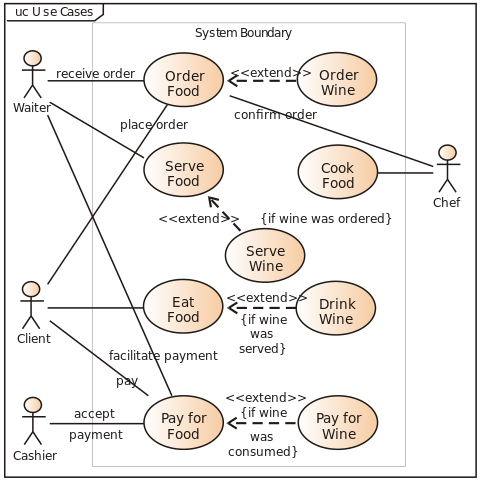
\includegraphics[width=0.8\linewidth]{figures/usecase.png}
  \caption{Use Case Diagram}
  \label{fig:flowchart}
\end{figure}
